\subsection{Semnalul video VGA}
\paragraph{}
Acesta este semnalul de la iesirea osciloscopului. Folosind un semnal VGA, osciloscopul construit in acest proiect poate fi conectat la orice monitor, si nu necesita unul incorporat. Semnalul VGA este usor de generat, iar majoritatea monitoarelor existente acum au conectori compatibili. In plus, construirea unui monitor integrat care sa afiseze semnalul este in afara scopului acestui proiect. Folosind un monitor extern osciloscopul nostru beneficiaza de o felxibiltate ridicata.

\begin{figure}[h]
\centering
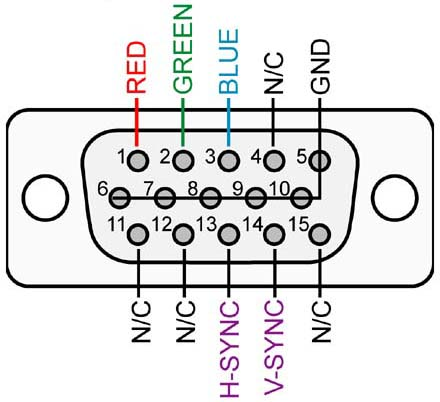
\includegraphics[width=120pt]{vga_pinout}
\caption{Conectorul VGA}
\label{fig:vga_pinout}
\end{figure}

\paragraph{}
Conectorul VGA utilizeaza 5 pini, dintre care 3 pentru culoare ( Rosu, Verde si Albastru ), impreuna cu 2 de sincronizare care reseteaza pozitia fascicolului de electroni pe verticala, respectiv orizontala. Valoarea tensiunii dintre fiecare pin pentru culoare si valoarea tensiunii pinului GND va determina intensitatea canalului respectiv. Pentru a intelege modul de utilizare al pinilor \emph{H-SYNC} si \emph{V-SYNC} trebuie sa intelegem mai intai modul de functionare a fascicolului de electroni in interiorul monitorului.

\begin{figure}[h]
\centering
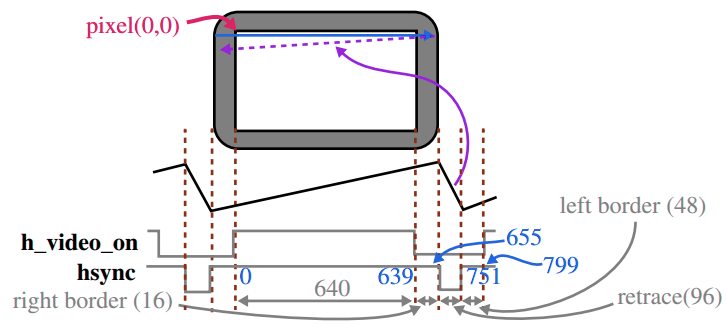
\includegraphics[width=290pt,height=120pt]{vga_timings}
\caption{Timpii de sincronizare VGA}
\label{fig:vga_timings}
\end{figure}

Fascicolul de electroni se misca cu viteza constanta de la stanga monitorului spre dreapta. Se observa totusi ca pozitia de incpeput a acestuia se afla inaintea zonei vizuale. Cand fascicolul de electroni se afla in stanga zonei vizuale, spunem ca se afla la marginea stanga. Definim in mod similar zona marginii drepte. Semnalul {\bf h\_video\_on } din Figura \ref{fig:vga_timings} are valoarea \emph{1} logic cand fascicolul de electroni se afla in zona vizuala, respectiv \emph{0} logic cand acesta se afla fie la marginea stanga, fie la marginea dreapta. Cand fascicolul a ajuns la capatul marginii drepte, se activeaza semnalul \emph{H-SYNC} pentru a incepe resetarea acestuia la marginea dreapta. In concluzie, fascicolul de electorni se poate afla in una din starile urmatoare:

\begin{enumerate}
\item{\bf marginea stanga} atunci cand se afla in stanga zonei vizuale
\item{\bf zona vizuala} cand fascicolul pargurge suprafata monitorului
\item{\bf marginea dreapta} cand fascicolul a depasit suprafata monitorului
\item{\bf curs de intoarcere} cand fascicolul este resetat la inceput
\end{enumerate}

Semnalul \emph{H-SYNC} trebuie sa fie tinut la valoarea \emph{0} in perioada a patra, cand fascicolul este in curs de intoarcere. In functie de rezolutia dorita, si frecventa monitorului, fiecare din aceste stari are o perioada fixa de timp. Semnalul \emph{V-SYNC} are acelasi rol, dar reseteaza fascicolul pe verticala. Deoarece ne vom referi la zonele din afara monitorului atat pe orizontala cat si pe verticala, le vom numi de acum inainte \emph{margine de inceput} si \emph{margine de sfarsit}. Ne vom referi la tabelul urmator pentru informatii despre timpi, considerand o rezolutie de {\tt 640x480}, si o frecventa de {\tt 60Hz}:

\begin{center}
    \begin{tabular}{| l | l | l |}
    \hline
    Stare & Timp Orizontala & Timp Verticala \\ \hline
	margine inceput & 16 & 10  \\ \hline
    zona vizuala & 640 & 480  \\ \hline
    margine sfarsit & 48 & 33 \\ \hline
    intoarcere & 96 & 2 \\ \hline
    total & 800 & 525 \\ 
    \hline
    \end{tabular}
\end{center}

Timpii sunt calculati in impulsuri de clock, iar frecventa clock-ului pentru un monitor de frecventa {\tt 60Hz} este {\tt 25.175MHz}.

\paragraph{}
Valorile semnalelor \emph{Red}, \emph{Green} si \emph{Blue} se schimba la fiecare impuls de clock cand fascicolul de electroni se afla in zona vizuala, pentru fiecare pixel in parte. Cand fascicolul se afla intr-una din marginile exterioare zonei vizuale sau se afla in starea de intoarcere, aceste semnale sunt setate la nivelul \emph{GND}.